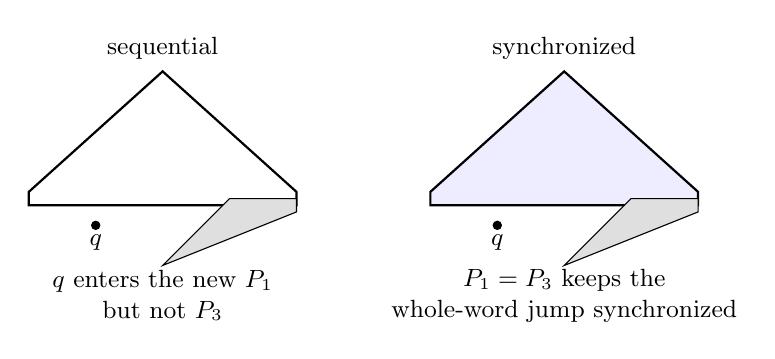
\begin{tikzpicture}[scale=.85,font=\small]
\begin{scope}
\draw[thick] (-2,0)--(2,0)--(2,.2)--(0,2)--(-2,.2)--cycle;
\draw[fill=gray!25] (0,-.9)--(1,.1)--(2,.1)--(2,-.1)--cycle;
\fill (-1,-.3) circle (2pt) node[below]{$q$};
\node at (0,2.35) {sequential};
\node[align=center] at (0,-1.35) {$q$ enters the new $P_1$\\but not $P_3$};
\end{scope}
\begin{scope}[xshift=6cm]
\draw[thick,fill=blue!7] (-2,0)--(2,0)--(2,.2)--(0,2)--(-2,.2)--cycle;
\draw[fill=gray!25] (0,-.9)--(1,.1)--(2,.1)--(2,-.1)--cycle;
\fill (-1,-.3) circle (2pt) node[below]{$q$};
\node at (0,2.35) {synchronized};
\node[align=center] at (0,-1.35) {$P_1=P_3$ keeps the\\whole-word jump synchronized};
\end{scope}
\end{tikzpicture}